\documentclass[11pt]{article}

\usepackage[T1]{fontenc}
\usepackage[utf8]{inputenc}
\usepackage{mathpazo}
\usepackage{amsmath,amssymb,amsthm,mathtools}
\usepackage[margin=1.05in]{geometry}
\usepackage{microtype}
\usepackage{enumitem}
\usepackage{booktabs}
\usepackage{xcolor}
\usepackage{titlesec}
\usepackage{fancyhdr}
\usepackage{tikz}
\usepackage{pgfplots}
\pgfplotsset{compat=1.17}
\usetikzlibrary{arrows.meta,positioning,calc,decorations.pathmorphing,backgrounds}
\usepackage{tcolorbox}
\tcbuselibrary{skins,breakable}
\usepackage[colorlinks=true,allcolors=accent]{hyperref}
\usepackage{url}
\urlstyle{same}

% ---------------------------------------------------------------- colours
\definecolor{accent}{HTML}{1D4E89}
\definecolor{accentlight}{HTML}{EAF0F7}
\definecolor{rule}{HTML}{C8D2DE}
\definecolor{warm}{HTML}{A8442A}
\definecolor{warmlight}{HTML}{FBF0EC}

% ---------------------------------------------------------------- headings
\titleformat{\section}{\large\bfseries\color{accent}}{\thesection.}{0.6em}{}
\titlespacing*{\section}{0pt}{1.6\baselineskip}{0.5\baselineskip}
\titleformat{\subsection}{\normalsize\bfseries}{\thesubsection}{0.6em}{}
\titlespacing*{\subsection}{0pt}{1.1\baselineskip}{0.35\baselineskip}

\pagestyle{fancy}
\fancyhf{}
\renewcommand{\headrulewidth}{0.4pt}
\renewcommand{\headrule}{\hbox to\headwidth{\color{rule}\leaders\hrule height \headrulewidth\hfill}}
\lhead{\footnotesize\color{accent}PHYS-GA 2043 \;\textbullet\; Machine Learning for Scientists}
\rhead{\footnotesize\color{accent}Lecture 2}
\cfoot{\footnotesize\thepage}

% ---------------------------------------------------------------- boxes
\newtcolorbox{keybox}[1][]{
  enhanced, breakable, colback=accentlight, colframe=accent,
  boxrule=0pt, leftrule=2.5pt, arc=1pt, left=10pt, right=10pt, top=7pt, bottom=7pt,
  fonttitle=\bfseries\color{accent}, coltitle=accent,
  attach boxed title to top left={yshift=-2mm,xshift=8pt},
  boxed title style={colback=accentlight,boxrule=0pt,arc=0pt},
  #1}

\newtcolorbox{asidebox}[1][]{
  enhanced, breakable, colback=warmlight, colframe=warm,
  boxrule=0pt, leftrule=2.5pt, arc=1pt, left=10pt, right=10pt, top=7pt, bottom=7pt,
  #1}

\newtcolorbox{algbox}[1]{
  enhanced, breakable, colback=white, colframe=rule, boxrule=0.6pt, arc=2pt,
  left=10pt, right=10pt, top=8pt, bottom=8pt,
  title={\color{accent}\bfseries #1}, fonttitle=\bfseries,
  colbacktitle=accentlight, coltitle=accent, titlerule=0pt,
  attach boxed title to top left={yshift=-2.6mm,xshift=10pt},
  boxed title style={boxrule=0pt,arc=1pt}}

% ---------------------------------------------------------------- macros
\DeclareMathOperator*{\argmin}{arg\,min}
\newcommand{\R}{\mathbb{R}}
\newcommand{\Loss}{\mathcal{L}}
\newcommand{\yhat}{\hat{y}}
\newcommand{\bs}[1]{\boldsymbol{#1}}
\newcommand{\board}[1]{\footnote{\textit{Board note:} #1}}

\setlist[itemize]{itemsep=2pt,topsep=4pt,leftmargin=1.4em}
\setlist[enumerate]{itemsep=2pt,topsep=4pt,leftmargin=1.7em}

\begin{document}

% ================================================================ TITLE
\begin{center}
{\color{accent}\rule{\textwidth}{1.2pt}}\\[9pt]
{\normalsize\color{accent}\scshape Lecture 2 \;\textbullet\; Thursday 10 September 2026}\\[8pt]
{\LARGE\bfseries Backpropagation and Loss Functions}\\[7pt]
{\large\itshape computing the gradient, and choosing what to minimise}\\[9pt]
{\normalsize Carolina Cuesta-Lazaro \;\textbullet\; PHYS-GA 2043}\\[6pt]
{\footnotesize\color{black!60} Transcribed and typeset by Claude from the lecture board notes}\\[8pt]
{\color{accent}\rule{\textwidth}{0.5pt}}
\end{center}

\vspace{0.2em}

% ================================================================ 1
\section{This week in AI4Science}

\begin{tcolorbox}[enhanced, colback=white, colframe=rule, boxrule=0.6pt, arc=2pt,
  left=10pt, right=10pt, top=7pt, bottom=7pt]
\small
\textbf{Links shown in class}
\begin{itemize}[leftmargin=1.2em, itemsep=1pt]
  \item T. Tao, \emph{Mathematics in the age of AI}, public lecture, ICM 2026 (slides) ---
        \url{https://teorth.github.io/tao-web/slides/age-of-ai-icm-2026.pdf}
  \item Written up as an essay --- \url{https://arxiv.org/abs/2608.16753}
\end{itemize}
\end{tcolorbox}

\noindent
Tao does not argue about whether AI can do mathematics. He assumes it can, as a working
hypothesis, and then asks the question he says the community has been avoiding: what are
the goals and values of mathematical research, including the implicit ones?

\medskip
\noindent
There are many reasons to do mathematics. To solve open problems, to build theories, to
understand the world, to build a community, to train the next generation, to make work of
lasting aesthetic value. Tao's central observation is that in the past these goals were
positively correlated. Progress on one usually meant progress on the others, so one could
be used as a proxy for the rest and most could be left unstated. His worry is that heavy
optimisation of a single goal, in particular by AI systems, can pull them apart. Solving
many problems very fast no longer implies that anyone understands the solutions, that they
have been checked, or that they have been absorbed into the field. He decomposes problem
solving into generation, verification, exposition, publication, digestion and
canonicalisation, and notes that AI accelerates the first stages while the later ones stay
slow and human. The result is a move from proof scarcity to proof abundance, with the
bottleneck shifting downstream.

\medskip
\noindent
The mechanism he appeals to is Goodhart's law: when a measure becomes a target, it stops
being a good measure. A proxy works only while it stays correlated with the thing you
actually care about, and optimising hard against the proxy is exactly what breaks the
correlation. The same question is worth asking about our own field, since the measures we
use in physics are proxies too.

% ================================================================ 2
\section{How do you compute a gradient?}
\label{sec:grad}

To run $\theta_{t+1} = \theta_t - \eta \nabla_\theta \Loss$ we need the gradient. The
question put to the class was how many ways of computing it we knew, and what each would
cost. Throughout, write $C$ for the cost of one forward pass $y = f_\theta(x)$ and $N$ for
the number of parameters. For a modern network $N$ is of order $10^{9}$.

\subsection*{1. Numerical differentiation}

Perturb one parameter at a time and take a finite difference:
%
\[
  \frac{\partial \Loss}{\partial \theta_i}
  \;\approx\;
  \frac{\Loss(\theta_i + \varepsilon) - \Loss(\theta_i)}{\varepsilon}.
\]
%
Each parameter needs its own forward pass, so the whole gradient costs
%
\[
  \text{cost} \;\sim\; N \cdot C \;\sim\; 10^{9}\,C .
\]
%
The accuracy is also poor. The truncation error is of order $\varepsilon$, which argues
for small $\varepsilon$, but the numerator is a difference of two nearly equal numbers, so
rounding error grows like $\epsilon_{\mathrm{mach}}/\varepsilon$, which argues for large
$\varepsilon$. The best you can do is around $\varepsilon \sim \sqrt{\epsilon_{\mathrm{mach}}}$,
which leaves roughly half your significant digits. This method is useful for checking a
gradient on a small model and for nothing else.

\subsection*{2. Symbolic differentiation}

Write the loss as one closed-form expression in $\theta$ and differentiate it with the
chain rule, as you would by hand:
%
\[
  \frac{\partial \Loss}{\partial \theta_L}(\theta_L),
  \qquad
  \frac{\partial x_L}{\partial \theta_{L-1}}(\theta_{L-1}),
  \qquad \ldots
\]
%
This is exact, but the expression for the derivative is much larger than the expression
for the function, and it grows with depth. The same subexpressions appear many times and
get recomputed. For a network of any realistic size the formula cannot be written down,
let alone evaluated efficiently.

\subsection*{3. Automatic differentiation}

\begin{keybox}
Automatic differentiation computes the full gradient, with respect to all $N$ parameters,
at a cost of about $2$--$3\,C$. The cost does not depend on $N$.
\end{keybox}

\noindent
This is the result that makes deep learning possible. Training a network with $10^{9}$
parameters costs roughly three forward passes per step, not $10^{9}$ of them.

% ================================================================ 3
\section{Autodiff and the computational graph}

Automatic differentiation is neither numerical nor symbolic. The idea is to stop treating
the function as one large formula and instead treat it as a graph of small operations,
called \emph{primitives}, each of which we know how to differentiate.

\begin{center}
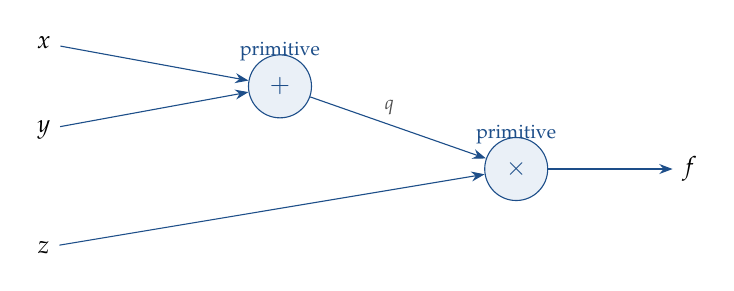
\begin{tikzpicture}[>=Stealth, node distance=10mm,
  op/.style={circle, draw=accent, fill=accentlight, minimum size=8mm, inner sep=0pt,
             font=\small, text=accent},
  var/.style={font=\small}]
  \node[var] (x) at (0,1.1) {$x$};
  \node[var] (y) at (0,0) {$y$};
  \node[var] (z) at (0,-1.5) {$z$};
  \node[op] (plus) at (3.0,0.55) {$+$};
  \node[op] (times) at (6.0,-0.5) {$\times$};
  \node[var] (f) at (8.2,-0.5) {$f$};
  \draw[->, accent] (x) -- (plus);
  \draw[->, accent] (y) -- (plus);
  \draw[->, accent] (plus) -- node[above, font=\scriptsize, black!70, pos=0.45] {$q$} (times);
  \draw[->, accent] (z) -- (times);
  \draw[->, accent] (times) -- (f);
  \node[font=\scriptsize, accent, above=2mm] at (plus) {primitive};
  \node[font=\scriptsize, accent, above=2mm] at (times) {primitive};
\end{tikzpicture}
\end{center}

\noindent
The graph above computes
%
\[
  q = x + y, \qquad f = q \cdot z .
\]
%
Each primitive has a local derivative we know in closed form:
$\partial q/\partial x = \partial q / \partial y = 1$, $\partial f/\partial q = z$ and
$\partial f/\partial z = q$. The derivative of the whole computation with respect to any
input is then a product of local derivatives along the path connecting them:
%
\[
  \frac{\partial f}{\partial y}
  = \frac{\partial f}{\partial q}\,\frac{\partial q}{\partial y} = z .
\]

\noindent
Backpropagation applies this rule once, working backwards from the loss through the graph.
Each intermediate derivative is computed once and reused by everything downstream of it,
rather than being recomputed for every parameter. That reuse is why the whole gradient
costs a small multiple of a single forward pass.

% ================================================================ 4
\section{Backpropagation in a deep network}

Write a network of $L$ layers as
%
\[
  z_\ell = W_\ell\, a_{\ell-1} + b_\ell,
  \qquad
  a_\ell = \sigma(z_\ell),
  \qquad \ell = 1, \ldots, L,
\]
%
with $a_0 = x$. Each layer does a linear map followed by an elementwise activation.

\begin{center}
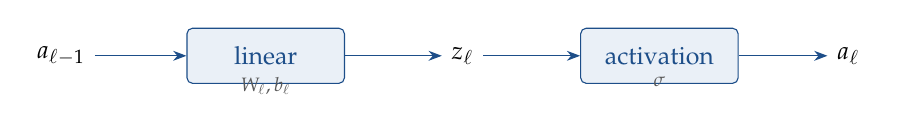
\begin{tikzpicture}[>=Stealth,
  blk/.style={draw=accent, fill=accentlight, rounded corners=2pt, minimum height=7mm,
              minimum width=20mm, font=\small, text=accent}]
  \node[font=\small] (ain) at (0,0) {$a_{\ell-1}$};
  \node[blk] (lin) at (2.6,0) {linear};
  \node[font=\small] (zl) at (5.1,0) {$z_\ell$};
  \node[blk] (act) at (7.6,0) {activation};
  \node[font=\small] (al) at (10.0,0) {$a_\ell$};
  \draw[->, accent] (ain) -- (lin);
  \draw[->, accent] (lin) -- (zl);
  \draw[->, accent] (zl) -- (act);
  \draw[->, accent] (act) -- (al);
  \node[font=\scriptsize, black!65, below=1.5mm] at (lin) {$W_\ell, b_\ell$};
  \node[font=\scriptsize, black!65, below=1.5mm] at (act) {$\sigma$};
\end{tikzpicture}
\end{center}

\noindent
Let $\delta_\ell = \partial\Loss/\partial z_\ell$ and let $D_\ell = \operatorname{diag}
\big(\sigma'(z_\ell)\big)$, the derivative of the activation at layer $\ell$. Applying the
chain rule layer by layer gives the backward recursion
%
\[
  \delta_L = D_L\,\frac{\partial \Loss}{\partial a_L},
  \qquad
  \delta_\ell = D_\ell\, W_{\ell+1}^{\top}\, \delta_{\ell+1},
  \qquad
  \frac{\partial \Loss}{\partial W_\ell} = \delta_\ell\, a_{\ell-1}^{\top}.
\]
%
Unrolling the recursion shows what the gradient at layer $\ell$ actually is:
%
\[
  \delta_\ell
  = D_\ell\, W_{\ell+1}^{\top}\, D_{\ell+1}\, W_{\ell+2}^{\top} \cdots
    W_{L}^{\top}\, D_L \; \frac{\partial \Loss}{\partial a_L}.
\]
%
It is a product of $L - \ell$ matrix factors, one pair per layer between $\ell$ and the
output. That product is where the next problem comes from.

% ================================================================ 5
\section{Vanishing and exploding gradients}

Take the typical size of one factor $D_k W_k^{\top}$ to be $\rho$. Then the size of the
gradient reaching layer $\ell$ behaves like
%
\[
  \|\delta_\ell\| \;\sim\; \rho^{\,L-\ell}.
\]
%
An exponential in depth has only two behaviours, and neither is what we want.

\begin{center}
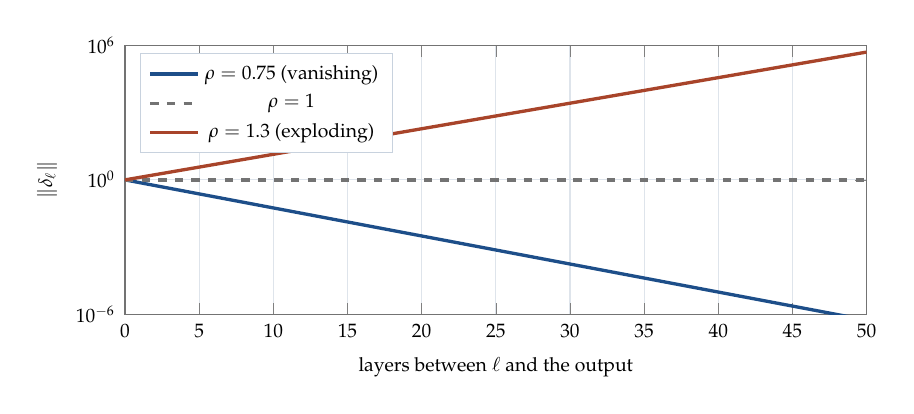
\begin{tikzpicture}
\begin{semilogyaxis}[
  width=11.0cm, height=5.0cm,
  xlabel={layers between $\ell$ and the output},
  ylabel={$\|\delta_\ell\|$},
  xmin=0, xmax=50, ymin=1e-6, ymax=1e6,
  label style={font=\scriptsize}, tick label style={font=\scriptsize},
  legend style={font=\scriptsize, draw=rule, at={(0.02,0.97)}, anchor=north west},
  grid=major, grid style={draw=rule!60},
  axis line style={draw=black!55}]
  \addplot[accent, very thick, domain=0:50, samples=60]{0.75^x};
  \addlegendentry{$\rho = 0.75$ (vanishing)}
  \addplot[black!55, very thick, dashed, domain=0:50, samples=60]{1};
  \addlegendentry{$\rho = 1$}
  \addplot[warm, very thick, domain=0:50, samples=60]{1.3^x};
  \addlegendentry{$\rho = 1.3$ (exploding)}
\end{semilogyaxis}
\end{tikzpicture}
\end{center}

\noindent
If $\rho < 1$ the gradient vanishes. The early layers receive essentially nothing and stop
learning, so a deep network trains only in its last few layers. If $\rho > 1$ the gradient
explodes, the updates are enormous and training diverges. Only $\rho \approx 1$ works, and
the deeper the network the more precisely that has to hold.

\medskip
\noindent
The sigmoid makes this worse. We saw in Lecture 1 that $\sigma' \le \tfrac14$, so every
$D_k$ contributes a factor of at most a quarter and vanishing is the default outcome. This
is one of the reasons ReLU, whose derivative is $0$ or $1$, replaced it.

\medskip
\noindent
Careful initialisation, normalisation layers and gradient clipping all help, but they are
adjustments to the size of the factors. The structural fix is to change what is being
multiplied.

% ================================================================ 6
\section{Residual connections}

Add the input of a block to its output:
%
\[
  a_\ell = a_{\ell-1} + f_\ell(a_{\ell-1}),
  \qquad\text{with, for example,}\quad
  f_\ell(a) = A(W a + b).
\]

\begin{center}
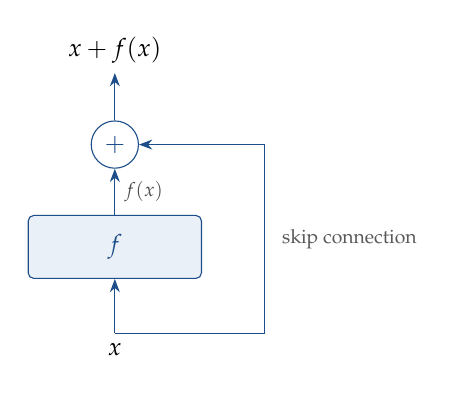
\begin{tikzpicture}[>=Stealth,
  blk/.style={draw=accent, fill=accentlight, rounded corners=2pt, minimum height=8mm,
              minimum width=22mm, font=\small, text=accent},
  sum/.style={circle, draw=accent, minimum size=6mm, inner sep=0pt, font=\small,
              text=accent}]
  \node[font=\small] (x) at (0,-2.2) {$x$};
  \node[blk] (f) at (0,-0.9) {$f$};
  \node[sum] (s) at (0,0.4) {$+$};
  \node[font=\small] (out) at (0,1.6) {$x + f(x)$};
  \draw[->, accent] (x) -- (f);
  \draw[->, accent] (f) -- node[right, font=\scriptsize, black!70] {$f(x)$} (s);
  \draw[->, accent] (s) -- (out);
  \draw[->, accent] (0,-2.0) -- (1.9,-2.0) -- (1.9,0.4) -- (s);
  \node[font=\scriptsize, black!65, right] at (2.0,-0.8) {skip connection};
\end{tikzpicture}
\end{center}

\noindent
The Jacobian of one block is now
%
\[
  \frac{\partial a_\ell}{\partial a_{\ell-1}} = \mathbb{I} + J_{f_\ell},
\]
%
and the Jacobian of the whole network is the product of these. Expanding that product is
what matters:
%
\[
  \prod_\ell \big(\mathbb{I} + J_{f_\ell}\big)
  = \mathbb{I}
  + \sum_\ell J_{f_\ell}
  + \sum_{\ell < \ell'} J_{f_{\ell'}} J_{f_\ell}
  + \cdots
\]

\begin{keybox}
Instead of a single product of $L$ factors, which is exponentially small or exponentially
large, the gradient is now a sum over all subsets of layers. The first term is the
identity: a path from the loss back to any layer that passes through no Jacobian at all.
The gradient can no longer vanish simply because the network is deep.
\end{keybox}

\noindent
There is a second reading of the same formula. At initialisation $f_\ell$ is small, so each
block is close to the identity and a deep residual network starts out behaving like a much
shallower one, becoming effectively deeper as training proceeds. This is why residual
networks train at hundreds of layers, and why essentially every modern architecture,
transformers included, is built from residual blocks.

\subsection*{Do they help with exploding gradients too?}

Only indirectly, and it is worth being clear about why. Taking norms in the product above,
%
\[
  \Big\| \prod_\ell \big(\mathbb{I} + J_{f_\ell}\big) \Big\|
  \;\le\; \prod_\ell \big(1 + \|J_{f_\ell}\|\big)
  \;=\; (1 + j)^{L}
  \qquad \text{if } \|J_{f_\ell}\| \sim j .
\]
%
This is still exponential in depth, and the base is now at least $1$. Residual connections
put a floor under the gradient but no ceiling on it: they remove the vanishing failure
mode and leave the exploding one. The same is true on the forward pass, where
$a_\ell = a_{\ell-1} + f_\ell(a_{\ell-1})$ makes the activations accumulate and grow with
depth.

\medskip
\noindent
What they do change is where the safe setting lies. In a plain network the signal has to
pass through every $W_\ell$, so the weights must be tuned so that $\rho \approx 1$: too
small and the signal dies, too large and it blows up, and the target gets narrower with
depth. In a residual network the identity already carries the signal, so the safe
configuration is simply $J_{f_\ell}$ small, with each block doing very little at first.
Making a residual branch small is easy, for instance by initialising its last layer near
zero or scaling it by $1/\sqrt{L}$. Making a product of matrices have singular values
close to $1$ is not.

\medskip
\noindent
Exploding gradients are then dealt with separately: normalisation layers inside the block
to hold the activations at a fixed scale, and gradient clipping, which rescales the update
whenever its norm exceeds a threshold.

% ================================================================ 7
\section{What loss should we use?}

So far $\Loss$ has been an unspecified scalar. We now ask what to put there.

\subsection*{Mean squared error}

The obvious choice is to penalise being wrong, and to penalise being more wrong more:
%
\[
  \Loss(\theta) = \frac{1}{N}\sum_{i=1}^{N}\big(\yhat_i - y_i\big)^{2},
  \qquad \yhat_i = f_\theta(x_i).
\]
%
This is the mean squared error, also called the L2 loss. It is smooth, differentiable
everywhere, always non-negative, and zero only when the prediction is exactly right. For a
linear model it is convex with a closed-form minimum. It is the default for regression and
it is what most people reach for without thinking about it.

\subsection*{L1, and what squaring does to outliers}

An equally reasonable choice is to penalise the error linearly:
%
\[
  \Loss(\theta) = \frac{1}{N}\sum_{i=1}^{N}\big|\,\yhat_i - y_i\,\big| .
\]
%
The two behave very differently in the presence of bad data. Under L2 an error of $10$
counts a hundred times an error of $1$, and its gradient contribution grows with the error,
so a single mislabelled point can dominate the total gradient and pull the fit towards
itself. Under L1 the derivative of $|\cdot|$ is $\pm 1$ however large the error is, so one
bad point contributes no more than any other. L1 is robust to outliers; L2 is not.

\medskip
\noindent
The price of L1 is that it is not differentiable at zero, and that its gradient does not
shrink as you approach the minimum, so the step size has to be decayed by hand.

\medskip
\noindent
So we have two defensible losses that give different answers on the same data. Choosing
between them by trial and error would be unsatisfying, and it turns out to be unnecessary:
these are not arbitrary ways of measuring distance, and each of them is answering a
specific question.

\subsection*{A problem where the answer is not unique}

Start from a real photograph of a face. Mask out the two boxes containing the eyes and
hand what is left to a network as its input $x$. The eyes are now gone, and many different
eyes are consistent with the rest of the face: looking left, looking right, open, half
closed. Nothing in the visible pixels picks one out.

\medskip
\noindent
If we could draw samples from the set of consistent completions, we would get a sequence of
sharp faces whose eyes move around inside those boxes. Train the same network with mean
squared error and we get one image, with a blurred smear where the eyes should be.

\noindent\begin{minipage}{\textwidth}\centering
\vspace{2pt}
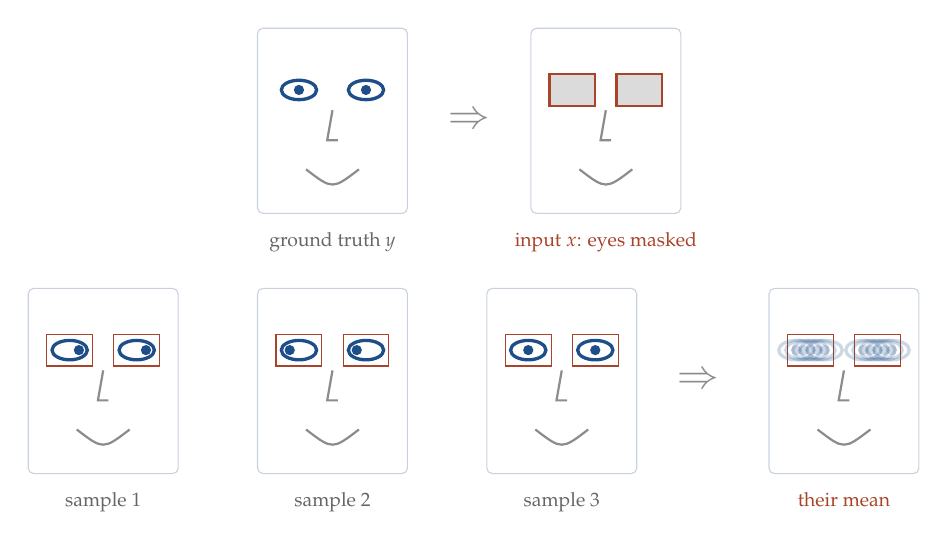
\begin{tikzpicture}[scale=1.12]
% ---------- row 1: ground truth and the masked input
\begin{scope}[shift={(2.6,2.95)}]
  \draw[rule, rounded corners=2pt] (-0.85,-1.05) rectangle (0.85,1.05);
  \draw[accent, very thick] (-0.38,0.35) ellipse [x radius=0.20, y radius=0.11];
  \draw[accent, very thick] ( 0.38,0.35) ellipse [x radius=0.20, y radius=0.11];
  \fill[accent] (-0.38,0.35) circle (0.058);
  \fill[accent] ( 0.38,0.35) circle (0.058);
  \draw[black!45, thick] (0,0.12) -- (-0.06,-0.22) -- (0.06,-0.22);
  \draw[black!45, thick] (-0.3,-0.55) .. controls (0,-0.78) .. (0.3,-0.55);
  \node[font=\scriptsize, black!60, below] at (0,-1.15) {ground truth $y$};
\end{scope}

\node[font=\Large, black!45] at (4.15,2.95) {$\Rightarrow$};

\begin{scope}[shift={(5.7,2.95)}]
  \draw[rule, rounded corners=2pt] (-0.85,-1.05) rectangle (0.85,1.05);
  \fill[black!14] (-0.64,0.17) rectangle (-0.12,0.53);
  \draw[warm, thick]  (-0.64,0.17) rectangle (-0.12,0.53);
  \fill[black!14] ( 0.12,0.17) rectangle ( 0.64,0.53);
  \draw[warm, thick]  ( 0.12,0.17) rectangle ( 0.64,0.53);
  \draw[black!45, thick] (0,0.12) -- (-0.06,-0.22) -- (0.06,-0.22);
  \draw[black!45, thick] (-0.3,-0.55) .. controls (0,-0.78) .. (0.3,-0.55);
  \node[font=\scriptsize, warm, below] at (0,-1.15) {input $x$: eyes masked};
\end{scope}

% ---------- row 2: posterior samples
\foreach \i/\dx/\ey in {1/0/0.105, 2/2.6/-0.105, 3/5.2/0.0}{
  \begin{scope}[shift={(\dx,0)}]
    \draw[rule, rounded corners=2pt] (-0.85,-1.05) rectangle (0.85,1.05);
    \draw[warm, thin] (-0.64,0.17) rectangle (-0.12,0.53);
    \draw[warm, thin] ( 0.12,0.17) rectangle ( 0.64,0.53);
    \draw[accent, very thick] (-0.38,0.35) ellipse [x radius=0.20, y radius=0.11];
    \draw[accent, very thick] ( 0.38,0.35) ellipse [x radius=0.20, y radius=0.11];
    \fill[accent] (-0.38+\ey,0.35) circle (0.058);
    \fill[accent] ( 0.38+\ey,0.35) circle (0.058);
    \draw[black!45, thick] (0,0.12) -- (-0.06,-0.22) -- (0.06,-0.22);
    \draw[black!45, thick] (-0.3,-0.55) .. controls (0,-0.78) .. (0.3,-0.55);
    \node[font=\scriptsize, black!60, below] at (0,-1.15) {sample \i};
  \end{scope}}

\node[font=\Large, black!45] at (6.75,0) {$\Rightarrow$};

% ---------- row 2: the mean
\begin{scope}[shift={(8.4,0)}]
  \draw[rule, rounded corners=2pt] (-0.85,-1.05) rectangle (0.85,1.05);
  \draw[warm, thin] (-0.64,0.17) rectangle (-0.12,0.53);
  \draw[warm, thin] ( 0.12,0.17) rectangle ( 0.64,0.53);
  \foreach \o in {-0.16,-0.08,0,0.08,0.16}{
    \draw[accent, opacity=0.22, very thick] (-0.38+\o,0.35)
         ellipse [x radius=0.20, y radius=0.11];
    \draw[accent, opacity=0.22, very thick] ( 0.38+\o,0.35)
         ellipse [x radius=0.20, y radius=0.11];
    \fill[accent, opacity=0.22] (-0.38+\o,0.35) circle (0.058);
    \fill[accent, opacity=0.22] ( 0.38+\o,0.35) circle (0.058);}
  \draw[black!45, thick] (0,0.12) -- (-0.06,-0.22) -- (0.06,-0.22);
  \draw[black!45, thick] (-0.3,-0.55) .. controls (0,-0.78) .. (0.3,-0.55);
  \node[font=\scriptsize, warm, below] at (0,-1.15) {their mean};
\end{scope}
\end{tikzpicture}
\vspace{4pt}
\end{minipage}

\medskip
\noindent
This is a documented effect and not an artefact of a weak network. In the super-resolution
literature the same observation was made explicitly: minimising the mean squared error
drives the model towards a pixel-wise average of the plausible solutions, which is smooth
and perceptually poor.\footnote{C.\ Ledig et al., \emph{Photo-realistic single image
super-resolution using a generative adversarial network}, arXiv:1609.04802; their
Figure~3 makes exactly this point.}

\medskip
\noindent
The lesson is that $y$ is not a function of $x$ here. What the data define is a conditional
distribution
%
\[
  p(y \mid x),
\]
%
the distribution over labels given the input.

\begin{asidebox}
\textbf{Prior and posterior.} $p(y)$ is the \emph{prior}: what images look like before we
observe anything, which the network learns implicitly from the training set. It is the
prior that knows faces have two roughly symmetric eyes. Observing $x$, the unmasked pixels,
updates it to the \emph{posterior} $p(y \mid x)$: the completions consistent with what we
can see, weighted by how plausible they were to begin with. Without a prior the problem is
hopeless, since any pixels at all are consistent with a masked region.
\end{asidebox}

\subsection*{If the likelihood were Gaussian}

Suppose we model that distribution as a Gaussian centred on the network output,
%
\[
  p(y \mid x) = \mathcal{N}\big(y; \, f_\theta(x), \, \sigma^{2}\big),
\]
%
which says the label is the prediction plus symmetric noise of the same width everywhere.
Its negative log-likelihood is
%
\[
  -\log p(y \mid x) \;=\; \frac{\big(y - f_\theta(x)\big)^{2}}{2\sigma^{2}}
                     \;+\; \log\!\big(\sigma\sqrt{2\pi}\big).
\]
%
With $\sigma$ fixed, the second term is a constant and the first is the squared error up to
a factor. Setting $\sigma = 1$,
%
\[
  -\log p(y \mid x) \;=\; \tfrac12 \big(y - \yhat\big)^{2} + \text{const},
\]
%
so minimising mean squared error \emph{is} maximum likelihood under a Gaussian of unit
width. The same calculation with a Laplace distribution in place of a Gaussian gives the L1
loss. The two losses from the start of this section are the negative log-likelihoods of two
different assumptions about the noise, which is the reason they disagree.

\subsection*{The result does not need that assumption}

It would be reasonable to conclude that the blurry face is the fault of the Gaussian
assumption, and that the fix is to assume something better. It is not. The derivation below
makes no assumption at all about $p(y \mid x)$ beyond its having a mean and a finite
variance.

\medskip
\noindent
Train with
%
\[
  \Loss(\theta) = \mathbb{E}_{x}\;
                  \mathbb{E}_{y \sim p(y|x)}\Big[ \big(\yhat - y\big)^{2} \Big],
  \qquad \yhat = f_\theta(x).
\]
%
Fix one value of $x$ and look at the inner expectation. With $x$ fixed, $\yhat$ is a
number, and the only random quantity is $y$. Define the mean of the posterior
%
\[
  \mu(x) \;=\; \mathbb{E}_{y \sim p(y|x)}[\,y\,] \;=\; \int y\, p(y \mid x)\, dy .
\]
%
Now add and subtract $\mu$ inside the square and expand:
%
\begin{align*}
  \mathbb{E}_{y}\big[(\yhat - y)^{2}\big]
  &= \mathbb{E}_{y}\Big[\big((\yhat - \mu) + (\mu - y)\big)^{2}\Big] \\[2pt]
  &= \underbrace{\mathbb{E}_{y}\big[(\yhat - \mu)^{2}\big]}_{\text{(i)}}
   + \underbrace{2\,\mathbb{E}_{y}\big[(\yhat - \mu)(\mu - y)\big]}_{\text{(ii)}}
   + \underbrace{\mathbb{E}_{y}\big[(\mu - y)^{2}\big]}_{\text{(iii)}} .
\end{align*}
%
Take the three terms in turn.

\begin{itemize}
  \item[(i)] Neither $\yhat$ nor $\mu$ depends on $y$, so the expectation does nothing and
  this term is just $(\yhat - \mu)^{2}$.
  \item[(ii)] Pull the constant factor $2(\yhat - \mu)$ out of the expectation, leaving
  $\mathbb{E}_{y}[\mu - y] = \mu - \mathbb{E}_{y}[y] = \mu - \mu = 0$. The cross term
  vanishes, and it vanishes precisely because $\mu$ was chosen to be the mean.
  \item[(iii)] This is $\mathbb{E}_{y}\big[(y - \mu)^{2}\big] = \operatorname{Var}[y \mid x]$,
  the spread of the posterior. It does not contain $\theta$ at all.
\end{itemize}

\begin{keybox}
\[
  \mathbb{E}_{y \sim p(y|x)}\Big[\big(f_\theta(x) - y\big)^{2}\Big]
  \;=\;
  \underbrace{\big(f_\theta(x) - \mu(x)\big)^{2}}_{\text{we control this}}
  \;+\;
  \underbrace{\operatorname{Var}[y \mid x]}_{\text{we do not}}
\]
The second term is a floor that no model can go below. The first is minimised, and equals
zero, when
\[
  f_\theta(x) \;=\; \mu(x) \;=\; \mathbb{E}[\,y \mid x\,].
\]
\end{keybox}

\noindent
Nothing in that calculation assumed the posterior was Gaussian. Whatever $p(y \mid x)$
actually is, bimodal or skewed or heavy-tailed, a network trained with mean squared error
converges to its mean. It is not learning to produce a plausible $y$; it is learning to
produce the average of all plausible $y$. For the masked face, the average of many sharp
faces whose eyes sit in different places is a blur. The blur is not a failure of the
network. It is the correct answer to the question we asked.

\medskip
\noindent
It is worth being explicit that the mean of a distribution need not be a plausible value
drawn from it. If the posterior has two modes, the mean sits between them, at a value the
posterior itself considers unlikely:

\begin{center}
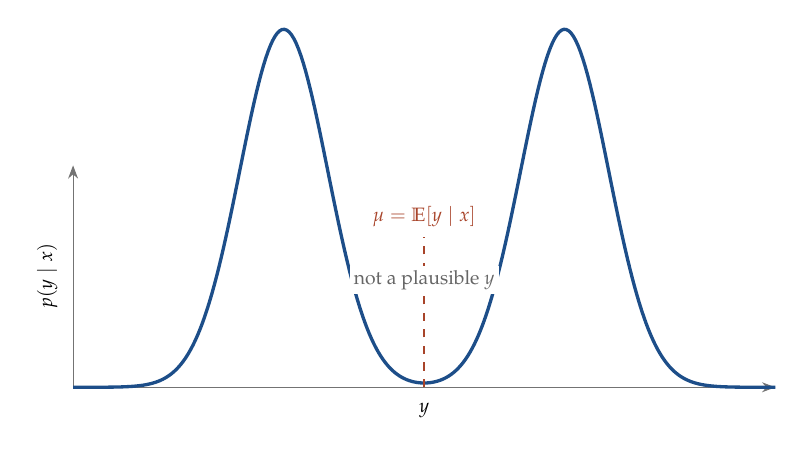
\begin{tikzpicture}
\begin{axis}[
  width=10.5cm, height=4.4cm,
  axis lines=left, xlabel={$y$}, ylabel={$p(y \mid x)$},
  label style={font=\scriptsize}, tick label style={font=\scriptsize},
  xtick=\empty, ytick=\empty,
  xmin=-4, xmax=4, ymin=0, ymax=0.62,
  axis line style={-Stealth, draw=black!55}, clip=false]
  \addplot[accent, very thick, samples=300, domain=-4:4]
    {exp(-(x+1.6)^2/0.5) + exp(-(x-1.6)^2/0.5)};
  \draw[warm, thick, dashed] (axis cs:0,0) -- (axis cs:0,0.42);
  \node[font=\scriptsize, warm, above] at (axis cs:0,0.42) {$\mu = \mathbb{E}[y \mid x]$};
  \node[font=\scriptsize, black!60, fill=white, inner sep=1.5pt] at (axis cs:0,0.30) {not a plausible $y$};
\end{axis}
\end{tikzpicture}
\end{center}

\noindent
The same derivation with an absolute value in place of a square returns the
\emph{median} of the posterior instead. That is the same robustness we saw earlier, seen
from the other side: the median ignores how far away the outliers are, and the mean does
not. But the median is still a single point estimate, so L1 does not solve the underlying
problem either.

\subsection*{Other losses}

Most of the losses we use are negative log-likelihoods of some assumed $p(y \mid x)$, and
each returns a different summary of the posterior.

\begin{center}
\small
\begin{tabular}{@{}lll@{}}
\toprule
\textbf{Loss} & \textbf{Assumed $p(y\mid x)$} & \textbf{What the optimum returns} \\
\midrule
$(\yhat - y)^{2}$ \; (L2, MSE) & Gaussian, fixed width & mean of the posterior \\
$|\yhat - y|$ \; (L1) & Laplace & median of the posterior \\
Cross entropy & categorical & the full posterior over classes \\
KL divergence, Wasserstein & --- & compare distributions, not points \\
Denoising loss & --- & the basis of diffusion and flow matching \\
\bottomrule
\end{tabular}
\end{center}

\noindent
Cross entropy is the interesting exception. For a discrete label the network can output a
probability for every class, so it represents the whole posterior rather than one number
summarising it. That is only possible because the label takes finitely many values.

% ================================================================ closing
\section*{Where this leaves us}

We now have the gradient, at a cost that does not grow with the number of parameters, and
residual connections to keep it from vanishing as the network gets deeper. The remaining
lesson is about what we ask the network to do. If the answer is genuinely uncertain, a
single output trained with mean squared error gives one summary statistic of the posterior
and has no way to express its spread. To obtain sharp, plausible answers we have to model
$p(y \mid x)$ itself and sample from it, which is what generative models do and where the
course goes later in the term.

\medskip
\noindent
Next lecture we turn to inductive biases and architectures: the MLP, convolutional
networks, graph networks and transformers.

\vspace{0.6em}
\noindent\textbf{\color{accent}Due Thursday 17 September.} Literature review: read between
five and ten papers in an area you are interested in, and for each write one sentence on
the main idea, one on something you would like to understand better, one on an experiment
you could run to build on it, and one on where you think there is a gap. Form your team.

\end{document}
